\documentclass[10pt,twocolumn,letterpaper]{article}

\usepackage{cvpr}
\usepackage{times}
\usepackage{epsfig}
\usepackage{graphicx}
\usepackage{amsmath}
\usepackage{amssymb}

% Include other packages here, before hyperref.

\usepackage{mathtools}
\DeclarePairedDelimiter\ceil{\lceil}{\rceil}
\DeclarePairedDelimiter\floor{\lfloor}{\rfloor}

\DeclareMathOperator*{\argmax}{argmax}
\DeclareMathOperator*{\argmin}{argmin}

\usepackage{algorithm}
\usepackage{algorithmic}

\usepackage{bbm}
\usepackage{xcolor}
\usepackage{booktabs} 
\def\BibTeX{{\rm B\kern-.05em{\sc i\kern-.025em b}\kern-.08em
    T\kern-.1667em\lower.7ex\hbox{E}\kern-.125emX}}
    
% \usepackage{subfig}
% \usepackage{subcaption}
\usepackage{subfigure}
\usepackage{bchart}

\usetikzlibrary{fit}

\makeatletter
\newdimen\legendxshift
\newdimen\legendyshift
\newcount\legendlines
% distance of frame to legend lines
\newcommand{\bclldist}{1mm}
\newcommand{\bclegend}[3][10mm]{%
    % initialize
    \legendxshift=0pt\relax
    \legendyshift=0pt\relax
    \xdef\legendnodes{}%
    % get width of longest text and number of lines
    \foreach \lcolor/\ltext [count=\ll from 1] in {#3}%
        {\global\legendlines\ll\pgftext{\setbox0\hbox{\bcfontstyle\ltext}\ifdim\wd0>\legendxshift\global\legendxshift\wd0\fi}}%
    % calculate xshift for legend; \bcwidth: from bchart package; \bclldist: from node frame, inner sep=\bclldist (see below)
    % \@tempdima: half width of bar; 0.72em: inner sep from text nodes with some manual adjustment
    \@tempdima#1\@tempdima0.5\@tempdima
    \pgftext{\bcfontstyle\global\legendxshift\dimexpr\bcwidth-\legendxshift-\bclldist-\@tempdima-0.72em}
    % calculate yshift; 5mm: heigt of bar
    \legendyshift\dimexpr7.5mm+#2\relax
    \legendyshift\legendlines\legendyshift
    % \bcpos-2.5mm: from bchart package; \bclldist: from node frame, inner sep=\bclldist (see below)
    \global\legendyshift\dimexpr\bcpos-2.5mm+\bclldist+\legendyshift
    % draw the legend
    \begin{scope}[shift={(\legendxshift,\legendyshift)}]
    \coordinate (lp) at (0,0);
    \foreach \lcolor/\ltext [count=\ll from 1] in {#3}%
    {
        \node[anchor=north, minimum width=#1, minimum height=5mm,fill=\lcolor] (lb\ll) at (lp) {};
        \node[anchor=west] (l\ll) at (lb\ll.east) {\bcfontstyle\ltext};
        \coordinate (lp) at ($(lp)-(0,5mm+#2)$);
        \xdef\legendnodes{\legendnodes (lb\ll)(l\ll)}
    }
    % draw the frame
    \node[draw, inner sep=\bclldist,fit=\legendnodes] (frame) {};
    \end{scope}
}
\makeatother

\usepackage{newfloat}
\DeclareFloatingEnvironment[
   fileext=loc
]{chart}

% If you comment hyperref and then uncomment it, you should delete
% egpaper.aux before re-running latex.  (Or just hit 'q' on the first latex
% run, let it finish, and you should be clear).
\usepackage[pagebackref=true,breaklinks=true,letterpaper=true,colorlinks,bookmarks=false]{hyperref}

\cvprfinalcopy % *** Uncomment this line for the final submission

\def\cvprPaperID{****} % *** Enter the CVPR Paper ID here
\def\httilde{\mbox{\tt\raisebox{-.5ex}{\symbol{126}}}}

% Pages are numbered in submission mode, and unnumbered in camera-ready
\ifcvprfinal\pagestyle{empty}\fi
\begin{document}

%%%%%%%%% TITLE
\title{Panoramic Video Separation with Online Grassmannian Robust Subspace Estimation}

\author{Kyle Gilman\qquad Laura Balzano\\Department of Electrical Engineering and Computer Science \\ University of Michigan \\ Ann Arbor, MI 48108 \\ email: \texttt{\{kgilman, girasole\}@umich.edu}}

\maketitle
\thispagestyle{plain}
\pagestyle{plain}
%\thispagestyle{empty}

%%%%%%%%% ABSTRACT
\begin{abstract}

In this work, we propose a new total variation (TV)-regularized robust principal component analysis (RPCA) algorithm for panoramic video data with incremental gradient descent on the Grassmannian. The resulting algorithm is competitive with state-of-the-art panoramic RPCA algorithms and can be computed frame-by-frame to separate foreground/background in video with a freely moving camera and heavy sparse noise.  Finally we compare foreground detection accuracy and computation time of our method versus several existing methods.
\end{abstract}

%%%%%%%%% BODY TEXT
\section{Introduction}

Video foreground/background separation is of great value to many computer vision algorithms for tasks such as activity or object recognition, target tracking, surveillance \cite{rpca_image_and_video_processiing}, or identifying trans-Neptunian objects in highly noisy astronomical data studies \cite{Gonzalez}. Modern applications such as these include a variety of challenges, ranging from video captured from consumer mobile devices to extremely memory-intensive video datasets. In this work, we focus on the problem of foreground/background separation in panoramic videos, where scalability with respect to memory and computation is a key requirement.

One successful collection of solutions for foreground/background separation in video leverages a problem formulation called robust principal component analysis (RPCA) \cite{wright2009robust}. RPCA naturally results in both foreground/background separation and foreground recovery. %RPCA algorithms estimate a low-rank subspace spanning the input data even in the presence of gross corruptions.
RPCA seeks to recover both a low-rank, incoherent matrix and a sparse corruptions matrix whose sum is the observed data \cite{Bouwmans_survey}. Such scenarios arise in many practical contexts where video data can be modeled as sparse foreground objects superpositioned on low-rank backgrounds. 

Most RPCA work in video separation has thoroughly addressed the case of static video, but modern video, especially from consumer mobile devices, often is captured by a camera undergoing motion, a significant challenge to models that assume a nearly constant background. More recent work on Panoramic RPCA \cite{B.Moore} has considered this issue, with the observation that panoramic video can be modeled as snapshots of small pieces of a large static scene with many missing pixels in each frame. However, this work as well as other existing RPCA methods become prohibitively expensive to compute in both time and memory with higher resolution videos and larger ranges of camera motion. The majority of batch algorithms use the singular value decomposition (SVD) to perform RPCA, but the SVD requires all of the data to be stored in memory at computation time and can be too slow for many real-time applications \cite{grasta}. The complexity of computing SVDs or thin SVDs grows quadratically in the number of matrix columns which may become prohibitive with large videos \cite{svd_cost}.

Finally, few RPCA models are capable removing sparse noise--or impulse noise--that cannot be distinguished from the foreground, such as in surveillance camera footage with blizzard or rainstorm conditions \cite{bad_weather_dataset} or in hyperspectral images \cite{Tariyal2016RemovingSN}. Video sequences are also often corrupted with inter-channel correlated impulse noise during the transmission stage, as a result of external effects such as thunderstorms, electric engines, wireless phones etc \cite{rodriguez_wohlberg}.


%\subsection{Contributions}
We propose a novel online RPCA algorithm that can handle panoramic camera motion. Our method is also robust to heavy sparse corruptions and can accurately disentangle the noise from foreground objects in the 2017 DAVIS Challenge videos \cite{DAVIS}. To the best of our knowledge, our method is the only one that can perform incremental gradient descent on the Grassmann manifold with total-variation (TV) regularization in an online way without using SVDs. We show our method is far more advantageous in computation time and memory than the existing state-of-the-art panoramic RPCA algorithm in \cite{B.Moore}.

\subsection{Organization}

The paper is organized as follows. In Section \ref{section:lit_review}, we briefly review existing RPCA algorithms in the literature and their models, advantages, and shortcomings. Section \ref{section:methods} formulates our proposed online Grassmannian model for panoramic robust PCA to handle video with free camera motion and sparse corruptions. We present our algorithms for solving the models and in Section \ref{section:experiments}, we provide the results of our experiments showing that our method is competitive with state-of-the-art algorithms. Finally Section \ref{section:conclusions} concludes and discusses opportunities for future work. 

%%%%%%%%%%%%%%%%%%%%%%%%%%%%%%%%%%%%%%%%%%%%%%%%%%%%%%%%
\section{Previous Work} \label{section:lit_review}

\subsection{RPCA Model in Video Decomposition}

Robust PCA algorithms are adept at low-rank-sparse decomposition in difficult problems with high-dimensional and incomplete data. Video background can be thought of as frames with high temporal correlation across the video. Mathematically, the matrix of vectorized video frames can be modeled as a rank-1 matrix $L = b \mathbbm{1}_n^T$ where $b \in \mathbb{R}^m$ is the vectorized background frame we wish to recover. While the matrix may not be exactly rank-1 empirically, it is usually very low-rank or close to rank-1. We seek to recover the low-rank subspace $U \in \mathbb{R}^{m \times r}$ and the weights $V^T \in \mathbb{R}^{r \times n}$ in the matrix factorization model $L = UV^T$ with $r \ll \min(m,n)$. Any foreground objects in each frame will appear as sparse corruptions in vectorized form added to the background frame. The observed video frame matrix $X \in \mathbb{R}^{m \times n}$ is then $X = L + S$ for some sparse matrix $S$.

\subsection{RPCA in Panoramic Video}

An abundance of research has developed algorithms capable of decomposing video where the background and camera are nearly static. The work in {\cite{candes}} proposed Principal Component Pursuit (PCP)--a classical batch RPCA algorithm that performs singular value shrinkage on the low-rank matrix component.  Other works have followed to further constrain the sparse foreground based on \textit{a priori} information. The authors of the Grassmannian Online Subspace Updates with Structured-sparsity (GOSUS) algorithm \cite{gosus} enforce the foreground objects to belong to superpixels, enhancing the cohesiveness and smoothness of foreground objects. However, the method is expensive to compute, requires a GPU solver, is slow to train, cannot separate the foreground from video corruptions like shotgun noise, and cannot handle missing data. 

The authors in \cite{tv_rpca} proposed to separate background from moving objects using TV-based regularization. It demonstrated TV-based models can effectively distinguish foreground, which should be smooth and spatially cohesive in image space, from sparse corruptions like snow and rain in poor weather conditions. Their method, called TVRPCA, composes the video as a summation of a low-rank component, a sparse TV-regularized foreground, and dense and sparse noise corruptions. TVRPCA is also a batch algorithm that uses the SVD for singular value shrinkage.

A far more challenging problem arises with nonstatic cameras. Researchers working on the DAVIS Challenge \cite{DAVIS} dataset seek to segment foreground objects in a large, diverse set of short, high-resolution RGB videos where the camera undergoes large degrees of motion. Moore, Gao, \& Nadakuditi \cite{B.Moore} showed a classic computer vision technique to re-register the frames into a common reference perspective where RPCA can be applied. Many of the videos in the DAVIS Challenge undergo perspective camera motion limited to eight degrees of freedom. Given correspondence points between frames, a homographic transformation between pairs of frames can be estimated. This clever preprocessing step allows RPCA to decompose the frames into a panoramic background component that spans the entire field of view. Unfortunately, this creates even higher-dimensional data when each transformed frame in the common reference perspective is vectorized. It also creates large numbers of unobserved pixels resulting from the partially overlapping views of the registered frames. This panoramic robust PCA (PRPCA) problem is the perfect storm of extremely high-dimensional and incomplete data.

The work in \cite{B.Moore} poses the video decomposition as a type of algorithm similar to TVRPCA. Their formulation is more advanced because it uses the OptShrink algorithm \cite{optshrink, Moore_Nadakuditi_Fessler} to update the low-rank subspace (which has been shown to be superior to singular value shrinkage algorithms) while separating the foreground from video corruptions like sparse and dense noise.

The GRASTA algorithm by He et al. \cite{grasta} models the background as a subspace on the Grassmann manifold and develops an iterative algorithm for tracking the low-rank subspace. GRASTA uses the natural $\ell_1$-norm cost function for data corrupted by sparse outliers, and operates only one data vector at a time, making it faster than other state-of-the-art algorithms and amenable to streaming and real-time applications \cite{grasta}. GRASTA uses explicit computations for the Grassmannian geodesics and the gradient of a function defined on the Grassmannian manifold in the work of Edelman, Arias and Smith \cite{edelman}. We will exploit a very similar Grassmannian update in our proposed methods.

GRASTA operates under the rank-sparsity model which assumes the foreground is sparse and its entries are distributed in a uniformly random pattern. This model works well in most instances, but it could further benefit from \textit{a priori} knowledge that the foreground objects are smooth and spatially cohesive in image space. This is especially complicated if the video is heavily corrupted by sparse noise. The rank-sparsity model is incapable of distinguishing between a sparse signal of interest and sparse corruptions, and foreground recovery is poor. We will show that our proposed algorithm inspired by GRASTA that we call PanGAEA (Panoramic Grassmannian Augmented Estimation Algorithm) not only achieves better foreground segmentations in clean video, but is also adept at handling sparse corruptions.

\section{Methods} \label{section:methods}
Our contribution is a novel Grassmannian descent algorithm that can handle missing data in panoramic video, operate orders of magnitude faster than batch methods, and can update its estimates with single streaming vectors in an online setting. We use the same panoramic mosaicking and preprocessing procedure as the authors in \cite{B.Moore}. Although the algorithm will be a batch method because of the homography registration, our Grassmannian algorithm still updates it estimates one data vector at a time in an online fashion.

\subsection{Registering two frames with a homography \cite{B.Moore}}

Given a point $p = [x,y,1]$ in a frame and its corresponding point $\tilde{p} = [\tilde{x},\tilde{y},1]$ in another frame, under the planar surface model, the points are related via the projective transformation

\begin{equation*}
	\kappa \tilde{p} = H^Tp
\end{equation*}

\noindent for some arbitrary nonzero scaling constant $\kappa$ and $H \in \mathbb{R}^{3\times3}$ with $H_{33}=1$. The homography matrix $H$ has eight unknown degrees of freedom we can estimate by minimizing 

\begin{equation} 	 \label{eq:homography}
	\min_h \|Ah\|^2 \quad \text{s.t.} \quad h_9 = 1
\end{equation}

\noindent where $h= \text{vec}(H)$, and given $c$ correspondences $\{p_i \mapsto \tilde{p}_i \}_{i=1}^c$, $A^T = [A_1^T, \ldots, A_c^T]$ where

\begin{equation*}
	A_i = \begin{bmatrix} 0 && p_i^T && -\tilde{y}_i p_i^T \\ p_i^T && 0 && -\tilde{x}_i p_i^T \end{bmatrix} \in \mathbb{R}^{2\times9}
\end{equation*}

To make the least squares problem well-conditioned, a minimum of four correspondence points is required, where each correspondence pair gives two independent linear equations and eight are needed to recover the eight unknown degrees of freedom. The solution to Eq. (\ref{eq:homography}) is the right-most singular vector of $A$ scaled so the last element is 1. This vector best approximates the vector in the null space of $A$ to minimize the objective in Eq.  (\ref{eq:homography}).

The correspondence points are also unknown, and we can use any popular computer vision feature algorithm, e.g. SIFT \cite{Lowe2004} or SURF \cite{SURF}, to find them and use RANSAC \cite{ransac} to robustly estimate the $H$ with the best objective value in (\ref{eq:homography}). Usually 10 correspondence points are best in each iteration of RANSAC to ensure a well-conditioned $A$.

\subsubsection{Homographic video registration}
The PRPCA problem registers each of the frames $F_1, \ldots, F_n \in \mathbb{R}^{a \times b}$ to the common reference. Like \cite{B.Moore}, we choose the middle frame $F_{\tilde{k}}$ as the ``anchor" frame, or the common reference, where $\tilde{k} = \floor{n/2}$. Each frame is highly correlated with the frame preceding and following it, so we can accurately estimate the homographies $H_k := H_{k \mapsto k+1}$ between frames $k$ and $k+1$. Let $\mathcal{H}_k := \mathcal{H}_{k+1}$ denote the linear transformation between all points in frames $k$ and $k+1$. Each transformed frame $\tilde{F}_k \in \mathbb{R}^{\tilde{a} \times \tilde{b}}$, where $\tilde{a}$ and $\tilde{b}$ are the height and width of the region defined by the union of the registered frame extents, can be computed with respect to the anchor frame by

\begin{equation}
	\tilde{F}_k = \begin{cases} (\mathcal{H}_{\tilde{k}-1} \circ \mathcal{H}_{\tilde{k}-2} \circ \ldots \circ \mathcal{H}_k)(F_k) &k<\tilde{k} \\
	F_k & k=\tilde{k} \\
	(\mathcal{H}_{\tilde{k}}^{-1} \circ \mathcal{H}_{\tilde{k}+1}^{-1} \circ \ldots \circ \mathcal{H}_{k-1}^{-1})(F_k) &k>\tilde{k}
	 \end{cases}
\end{equation}

We then construct our data matrix $X \in \mathbb{R}^{m \times n}$ for the RPCA problem where $m = \tilde{a}\tilde{b}$ as 

\begin{equation}
	X = [\text{vec}(\tilde{F}_1) \ldots \text{vec}(\tilde{F}_p)]
\end{equation}

As an example, we illustrate the homographic frame registration result for ``Horsejump-High" from the DAVIS Challenge \cite{DAVIS} in Fig. \ref{fig:horsejump_registration}. The horse and jockey jump over the gate and gallop towards the red gate seen at the right. Here, each frame has been transformed to a global coordinate system in reference to the video's anchor frame and overlain in reverse sequence.

Following panoramic transformation, the moving camera video data is expressed as a static space-time matrix where each row corresponds to a fixed point in space and where missing matrix entries are unobserved pixels of the panoramic mosaic scene \cite{B.Moore}. We then perform RPCA on the registered frames matrix with our fast Grassmannian stochastic gradient descent algorithm.

\begin{figure}
    \centering
    \includegraphics[width=0.48\textwidth]{pano_img.jpg}
    \caption{Frames of the video ``Horsejump-high" registered in panoramic mosaic.}
    \label{fig:horsejump_registration}
\end{figure}



%%%%%%%%%%%%%%%%%%%%%%%%%%%%%%%% 
\subsection{Model and Algorithms}

We propose our algorithm called PanGAEA that adheres to rank-sparsity theory for well-posed separability while regularizing the foreground with TV smoothing. This should not only improve segmentation generally but also make the segmentation robust to sparse noise.

PanGAEA is motivated from TVRPCA \cite{tv_rpca} and GRASTA \cite{grasta} to obtain fast video separation using iterative Grassmannian descent with TV-regularization of the foreground vector in the objective function. We first model the batch problem using all $n$ frames of the video $X \in \mathbb{R}^{m \times n}$ for vectorized frames of ambient dimension $m$:

\begin{equation}
    \begin{split}
        \min_{U, W, S, E} \quad &  \text{TV}(S) + \beta_S\|S\|_1 + \|E\|_1 \\
    \text{s.t. } & \mathcal{A}_\Omega (X) = \mathcal{A}_\Omega (UW + S + E) \\
    & U^T U = I 
    \end{split}
    \label{eq:pangaea_global}
\end{equation}

\noindent Above, $\|Y\|_1 = \sum_{i,j} |Y_{ij}|$ for some $m \times n$ matrix $Y$. The linear operator $\mathcal{A}_\Omega(\cdot)$ extracts the pixels observed in the panorama mosaic scene on the set $\Omega \subset \{1,\hdots,m\} \times \{1,\hdots, n\}$. We assume all original frame pixels are observed. $U \in \mathbb{R}^{m \times r}$ is the orthonormal matrix whose columns span the rank-$r$ subspace from which the background frames approximately lie in. We say that $U$ is a point on the Grassmann manifold of subspaces, denoted $U \sim \mathcal{G}(m,r)$, which is the set of all subspaces of dimension $r$ in $\mathbb{R}^{m}$. The Grassmannian is a compact Riemannian manifold, and its geodesics can be explicitly computed \cite{grouse}.

The matrix $W \in \mathbb{R}^{r \times n}$ is the weights matrix. The matrix $S \in \mathbb{R}^{m \times n}$ captures the sparse foreground objects, and $E \in \mathbb{R}^{m \times n}$ models sparse corruptive noise. The hyperparameter $\beta_S$ balances the smoothness of the foreground signal with the sparsity of the noise. Here $\text{TV}(S) = \|WCS\|_1$ where $C$ is the block-circulant first-order differences matrix formed by

\begin{equation}
	C \in \mathbb{R}^{2m \times m} = \begin{bmatrix} I_N \otimes D_M \\ D_N \otimes I_M \end{bmatrix}
\end{equation}

\noindent Here, $D_M$ is the $M \times M$ first-order differences matrix. Recall that $M,N$ are the dimensions of the registered frames in the common reference. $W$ is the square, diagonal matrix of weights whose diagonal $d$ has zeros on the indices corresponding to the circulant boundaries and ones otherwise.

We rewrite the problem in Eq. (\ref{eq:pangaea_global}) in terms of each frame, or column, at time instance $t$ where each column is observed on the set $\Omega_t \subset \{1,\hdots,m\}$ for $n=T$ columns:

\begin{equation}
    \begin{split}
        \min_{s_{t},e_t,U_t,w_t} & \sum_{t=1}^T  \|WC\chi_{\Omega_t}(s_{\Omega_t})\|_1 + \beta_S \|s_{\Omega_t}\|_1 + \|e_{\Omega_t}\|_1  \\
	\text{s.t. } & x_{\Omega_t}= U_{\Omega_t}w_t + s_{\Omega_t} + e_{\Omega_t} \\
	&U_t^T U_t = I 
    \end{split}
\end{equation}

\noindent Here, $U_{\Omega_t}$ denotes the $|\Omega_t| \times r$ submatrix formed by extracting the rows indexed observed on $\Omega_t$, and similarly for $x_{\Omega_t}, s_{\Omega_t},$ and $e_{\Omega_t}$. We also denote the linear operator $\chi_{\Omega_t}(\cdot)$ which zero pads a vector argument of length $|\Omega_t|$ to dimension $m$ on the indices in the complement of $\Omega_t$. We then minimize this objective function with a stochastic gradient descent procedure for each time instance $t$:

\begin{equation}
\begin{split}
	\min_{s_{t},e_t,U_t,w_t} & \|WC\chi_{\Omega_t}(s_{\Omega_t})\|_1 + \beta_S\|s_{\Omega_t}\|_1 +  \|e_{\Omega_t}\|_1  \\
	\text{s.t. } & x_{\Omega_t}= U_{\Omega_t}w_t + s_{\Omega_t} + e_{\Omega_t} \\
	&U_{t}^T U_{t} = I 
\end{split}
\label{eq:pangaea_objective}
\end{equation}

Note that we have enforced the foreground in $s_t$ to be TV-smooth in image space but also sparse. While Moore, Gao, \& Nadakuditi \cite{B.Moore} argue the sparsity constraint is over-restrictive, we found it was actually necessary in our model to be accountable to rank-sparsity theory and achieve any kind of acceptable separation. The two regularizers work in concert to separate foreground objects that are recoverable in the RPCA sense, but also conform to our heuristical understanding of how foreground objects should appear and behave in video. 

To make the terms in the objective function of (\ref{eq:pangaea_objective}) separable in each variable and compatible with the ADMM model, we can rewrite the problem using linear constraints as 

\begin{equation}
\begin{split}
	\min_{z_{t},s_{t},\xi_t,e_{t},U_{t},w_t} & \|Wz_t\|_1 + \beta_S\|\xi_{\Omega_t} \|_1+ \|e_{\Omega_t}\|_1 \\
	\text{s.t. } &z_t = C\chi_{\Omega_t}(s_{\Omega_t}) \\
	& x_{\Omega_t} = U_{\Omega_t}w_t + \xi_{\Omega_t} + e_{\Omega_t} \\
	& \xi_{\Omega_t} = s_{\Omega_t} \\
	&U_{t}^T U_{t} = I \\
\end{split}
\label{eq:pangaea_objective2}
\end{equation}

\noindent with $z_t \in \mathbb{R}^{2m}, x_t, s_t,\xi_t,e_t \in \mathbb{R}^m,$ and $w_t \in \mathbb{R}^r$.  The problem is nonconvex because of the coupling between $U_t$ and $w_t$ and because $U_t$ lies on the Grassmann manifold. First, we form the augmented Lagrangian and optimize by block-coordinate descent. We alternate by holding $U_t$ fixed and solving for the variables $z_{t},s_{t},\xi_t,e_{t},$ and $w_t$ with ADMM; then, holding all variables fixed except for $U_t$, our algorithm takes a geodesic step along the manifold in the direction of the negative gradient of the augmented Lagrangian. 

From Eq. (\ref{eq:pangaea_objective2}), we form the augmented Lagrangian with the dual variables of appropriate dimensions ${\lambda_1}_t, {\lambda_2}_t,$ and ${\lambda_3}_t$ at time $t$. After completing the square and ignoring constant terms, the augmented Lagrangian becomes

\begin{equation}
\begin{split}
	&\mathcal{L}(U_t,z_t,s_t,\xi_t,e_t,w_t,\lambda_{{1,2,3}_t}) = \\
	& \|Wz_t\|_1 +  \beta_S\|\xi_{\Omega_t}\|_1 + \|e_{\Omega_t} \|_1 \\
	&+  \frac{\rho_1}{2}\|C\chi_{\Omega_t}(s_{\Omega_t}) - z_t + \frac{\lambda_{1_t}}{\rho_1}\|_2^2 + \frac{\rho_2}{2} \|\xi_{\Omega_t} - s_{\Omega_t} + \frac{\lambda_{2_t}}{\rho_2} \|^2_2  \\
	&+ \frac{\rho_3}{2}\|U_{\Omega_t}w_t + \xi_{\Omega_t} + e_{\Omega_t} - x_{\Omega_t} + \frac{\lambda_{3_t}}{\rho_3}\|^2_2 \end{split}
	\label{eq:augmented_lagrangian}
\end{equation}

\noindent The smoothing penalties $\rho$ are user-defined, and we will assume all three penalties are equal to 1.8, which works well in practice.

\subsubsection{Updates of the principal weights, sparse vectors, surrogate variables, and dual variables with ADMM}

Given an estimate of the subspace $\hat{U}_t$, the problem in (\ref{eq:pangaea_objective2}) is a constrained convex optimization problem with strong duality \cite{boyd:cvx_opt}. Given the partial observation $x_{\Omega_t}$ and the observed entries’ indices $\Omega_t$, the optimal $(z_t^*, s_t^*,\xi_t^*,e_t^*,w_t^*,\lambda^*_{{1,2,3}_t})$ in Eq. (\ref{eq:pangaea_objective}) can be found by minimizing the augmented Lagrangian in Eq. (\ref{eq:augmented_lagrangian}) with respect to these variables:

\begin{equation}
\begin{split}
	(z_t^*, s_t^*,&\xi_t^*,e_t^*,w_t^*,\lambda^*_{{1,2,3}_t}) = \\
	 &\argmin_{z_t, s_t,\xi_t,e_t,w_t,\lambda_{{1,2,3}_t}} \mathcal{L}(\hat{U}_t, z_t, s_t,\xi_t,e_t,w_t,\lambda_{{1,2,3}_t})
\end{split}
\label{eq:argmin_aug_Lagrangian}
\end{equation}

We efficiently update each variable in Eq. (\ref{eq:argmin_aug_Lagrangian}) with ADMM in an alternating fashion, yielding the updates given in Steps (5) and (6) of Algorithm \ref{alg:pangaea_admm}.

We note that $z = \text{S}_\beta(y) = \text{sign}(y) \odot \max(|y| - \beta, 0)$ in Algorithm \ref{alg:pangaea_admm} is the elementwise soft-thresholding operator of argument vector $y \in \mathbb{R}^d$ for some positive constant $\beta$ that yields the vector $z \in \mathbb{R}^d$ \cite{Beck2009AFI,fessler_lrmc}. 

The matrix-vector product $C \chi_{\Omega_t}(s_{\Omega_t})$ in Algorithm \ref{alg:pangaea_admm} can be efficiently computed by taking the first order differences of only the observed pixels in the frame. We also assume above that the matrix $U_{\Omega_t}^TU_{\Omega_t}$ is always invertible, which has been shown to be guaranteed if $|\Omega_t|$ is large enough \cite{balzano_recht}. 

The derived update of $s_t$ originally involves the inverse of a very large matrix $(I + C^TC) \in \mathbb{R}^{m \times m}$, assuming all $\rho$'s are equal. Computing the inverse is prohibitive for our applications in video where $m$ is usually very large. Fortunately, the matrix has block-circulant structure and can be shown to have a very fast and efficient update that does not involve difficult matrix inverses \cite{bcirculant_matrices}:

\begin{equation}
 s_{t}^{k+1}= \mathcal{F}^{-1}_2 \left (\frac{\mathcal{F}_2(\rho_1 C^T(z_t^k - \lambda_{1_t}^k/\rho_1) + \rho_3r_t^{k+1})}{1 + \rho_1 \mathcal{F}_2(c)} \right ) 
\end{equation}

\noindent where $\mathcal{F}_2 : \mathbb{R}^{MN} \rightarrow \mathbb{R}^{MN}$ (again, $M,N$ are the dimensions of the registered frames in the common reference, and where the ambient dimension of the video data becomes $m = MN$) denotes the operator that reshapes its input into an $M \times N$ matrix, computes the 2D fast Fourier transform, and vectorizes the result. The vector $c =C^TC[:, 1]$ denotes the first column of the matrix $C^TC$. This denominator is a constant and can be precomputed.  The total computational complexity of one update is dominated by the Fourier updates at $O(m\log(m))$. ADMM empirically converges very quickly, usually within a few tens of iterations. In our algorithm, we found 50 iterations to work well for high-dimensional video to where the Karush-Kuhn Tucker (KKT) conditions are met within precision of some small $\epsilon$. 

\subsubsection{Grassmannian geodesic gradient step}
The partial derivative of the augmented Lagrangian with respect to the components of $U$ given estimates of the other variables from ADMM is

\begin{equation}
	\frac{\partial \mathcal{L}}{\partial U} = \chi_{\Omega_t}({\lambda_3}_t^* + \rho_3(U_{\Omega_t} w_t^* + + \xi_{\Omega_t}^*+ e_{\Omega_t}^* - x_{\Omega_t}){w^*_t}^T)
\end{equation}

From the work of \cite{edelman}, the gradient of the augmented Lagrangian on the Grassmannian is

\begin{equation}
	 \nabla  \mathcal{L} = (I - UU^T)\frac{\partial \mathcal{L}}{\partial U} = \Gamma {w^*_t}^T
\end{equation}

where

\begin{equation}
\begin{split}
	\Gamma_1 &= {\lambda_3}_t^* + \rho_3(U_{\Omega_t} w_t^* + \xi_{\Omega_t}^* + e_{\Omega_t}^*  - x_{\Omega_t})\\
	\Gamma_2 &= U_{\Omega_t}^T \Gamma_1\\
	\Gamma &= \chi_{\Omega_t} \Gamma_1 - U\Gamma_2
\end{split}
\label{eq:gamma}
\end{equation}

It is easily verified that $\nabla \mathcal{L}$ is a rank-1 matrix with a trivial SVD whose only nonzero singular value is $\sigma = \|\Gamma\| \|w^*_t\|$ with left and right singular vectors  $\Gamma/\|\Gamma\|$ and ${w^*_t}/\|w^*_t\|$ respectively. From \cite{edelman}, the gradient step on the Grassmann manifold for some positive length $\eta$ in the direction of $-\nabla  L$ is

\begin{equation}
\small
	U_{t+1}(\eta) = U_t + \left ((\cos(\eta \sigma) - 1) \frac{U_tw_t^*}{\|w_t^*\|} - \sin(\eta \sigma) \frac{\Gamma}{\|\Gamma\|}\right )\frac{{w^*_t}^T}{\|w_t^*\|}
	\label{eq:subspace_update}
\end{equation}

PanGAEA is fully summarized in Algorithm \ref{alg:pangaea}.

\subsubsection{Complexity Analysis}

The total cost of PanGAEA is $O(|\Omega|r^3 + Km\log(m) + K|\Omega|r + mr^2)$. Algorithm \ref{alg:pangaea} costs $O(|\Omega |r^3 + |\Omega| r + mr^2)$ flops like GRASTA. The $w_t$ and soft-thresholding updates in the ADMM solver in Algorithm \ref{alg:pangaea_admm} are simple linear algebraic computations and require at most $O(K|\Omega|r)$ flops. A notable advantage of PanGAEA is its savings in these updates from operating on dimensions $|\Omega|$, the number of observed pixels, compared to the full ambient dimension $m$. The update for $s_t$ is the most costly in the ADMM solver, requiring $O(Km\log(m))$. PanGAEA also avoids computing SVDs, a cost which grows quadratically in the number of video frames. PanGAEA relies on simple, efficient linear algebra operations with linear complexity in the data dimensions, is constant in memory use, and is numerically stable by maintaining orthonormality on the Grassmann manifold. 

\begin{algorithm}
 \caption{Algorithm for PanGAEA}
 \begin{algorithmic}[1]
 \renewcommand{\algorithmicrequire}{\textbf{Input:}}
 \renewcommand{\algorithmicensure}{\textbf{Output:}}
 \REQUIRE A $m \times r$ orthonormal matrix $U_0$. A sequence of corrupted vectors $x_t$, each vector observed in entries $\Omega_t \subset \{1, . . . , m\}$. Step size $\eta > 0$. Regularizer $\beta_S > 0$. Augmented Lagrangian penalty $\rho$.
 \ENSURE  $U_t$ and $w_t, s_t, e_t$ at time $t$.
 \STATE Form $C = \begin{bmatrix} I_N \otimes D_M & D_N \otimes I_M  \end{bmatrix}^T$
 \STATE Compute $c = C^TC[:,1]$
 \STATE Compute $\phi = 1 + \rho \mathcal{F}_2(c)$
  \FOR {$t = 0$ to $T$}
  \STATE Extract $U_{\Omega_t}$ from $U_t$: $U_{\Omega_t} = \mathcal{A}_{\Omega_t}(U_t)$
  \STATE Estimate $w_t^*,s_t^*, \xi_t^*,e_t^*,{\lambda_3}_t^*$ via Algorithm \ref{alg:pangaea_admm}.
  \STATE Compute $\Gamma$ by Eq. (\ref{eq:gamma}).
\STATE Update the subspace with Eq. (\ref{eq:subspace_update}).
  \ENDFOR
 \RETURN $U_{t+1}$ and $w_t, s_t, e_t, \quad \forall t = 0, \ldots, T$
 \end{algorithmic} 
 \label{alg:pangaea}
 \end{algorithm}
 
 \begin{algorithm}
 \caption{ADMM Solver for PanGAEA}
 \begin{algorithmic}[1]
 \renewcommand{\algorithmicrequire}{\textbf{Input:}}
 \renewcommand{\algorithmicensure}{\textbf{Output:}}
 \REQUIRE A $|\Omega_t| \times r$ orthonormal matrix $U_{\Omega_t}$. A sequence of corrupted vectors $x_t$, each vector observed in entries $\Omega_t \subset \{1, . . . , m\}$. Augmented Lagrangian penalty $\rho$. Parameter $\mu_0$. Denominator of $s$ update $\phi$. Tolerance $\epsilon$.
 \ENSURE  $w_t, s_t, e_t$ at time $t$.
 \STATE Precompute $P = (U_{\Omega_t}^TU_{\Omega_t})^{-1}{U_{\Omega_t}}^T$
 \STATE $\mu^k = \mu_0$
  \FOR {$k = 0$ to $K$ or until convergence}
   \STATE Update principal weights: \\
   $w^{k+1} = P(x_{\Omega_t} -\xi_{\Omega_t}^k - e_{\Omega_t} ^k- \lambda_{3}^k/\mu^k)$
   \STATE Update foreground sparse vector: \\
   $r^{k+1} = \chi_{\Omega_t}(\xi_{\Omega_t}^k+ \lambda_{2}^k/\mu^k)$\\
    $s^{k+1}= \mathcal{F}^{-1}_2(\frac{\mathcal{F}_2(\mu^k C^T(z^k - \lambda_{1}^k/\mu^k) + \mu^k r^{k+1})}{\phi}) $
   \STATE Update soft-thresholded variables: \\
   $h^{k} = x_{\Omega_t} - U_{\Omega_t}w^{k+1} - \lambda_{3}^k/\mu^k$ \\
    $\xi_{\Omega_t}^{k+1} = \frac{1}{2} \text{S}_{\beta_S/\mu^k}(h^{k} - e_{\Omega_t}^k + s_{\Omega_t}^{k+1} -\lambda_{2}^k/\mu^k)$ \\
    $e_{\Omega_t}^{k+1} = \text{S}_{1/\mu^k}(h^{k} - \xi_{\Omega_t}^{k+1})$ \\
    $z^{k+1} = \text{S}_{d./\mu^k}(C\chi_{\Omega_t}(s_{\Omega_t})^{k+1} + \lambda_{1}^k/\mu^k)$ 
   \STATE Update the residuals of the linear equality constraints: \\
   $y_1^k = C \chi_{\Omega_t}(s_{\Omega_t}^{k+1}) - z^{k+1}$ \\
   $y_2^k = U_{\Omega_t}w^{k+1} + \xi_{\Omega_t}^{k+1} + e_{\Omega_t}^{k+1}  - x_{\Omega_t}$ \\
   $y_3^k = \xi_{\Omega_t}^{k+1} - s_{\Omega_t}^{k+1} $
   \STATE Update the dual variables \\
   	$\lambda_{1}^{k+1} = \lambda_{1}^k + \mu^k y_1^k $ \\
	$\lambda_{2}^{k+1} = \lambda_{2}^k + \mu^k y_2^k $ \\
	$\lambda_{3}^{k+1} = \lambda_{3}^k + \mu^k y_3^k$
\STATE Update the ADMM penalty $\mu^{k+1} = \rho \mu^k$
\IF{$\max \{\|y_1\|_2, \|y_2\|_2, \|y_3\|_2 \} \leq \epsilon$}
	\STATE Converge and break the loop
\ENDIF
  \ENDFOR
 \RETURN $w_t^* = w^{k+1}, s_t^* = s^{k+1}, e_t^* = e^{k+1}$
 \end{algorithmic} 
 \label{alg:pangaea_admm}
 \end{algorithm}

\section{Experiments \& Evaluation} \label{section:experiments}

\subsection{DAVIS Challenge Video Separation}

Next we show experimental results of our algorithms on RGB frames of the DAVIS Challenge \cite{DAVIS} compared to RPCA with OptShrink \cite{candes, B.Moore}, GRASTA \cite{grasta}, and PRPCA \cite{B.Moore}. The DAVIS Challenge provides ground-truth binary masks of the foreground objects in each video frame, and we will use these masks to compute the receiver operating characteristic (ROC) curves of each algorithm by measuring the true positive and false positive rates.

We also measure the mean peak signal-to-noise ratios (PSNR) for each algorithm's denoised frames--the sum of the recovered background and foreground frames--with reference to the original frame in Table \ref{tab:psnrs}. Lastly, we show the significant computational speedup of our Grassmannian stochastic gradient descent approach for each DAVIS video in Chart \ref{fig:comp_times} which displays the total computation times for each algorithm.

Both Grassmannian algorithms are specified to learn a rank-1 subspace. We found that $\beta_S = 0.5$ worked well in PanGAEA. We run PanGAEA for 7 epochs, randomly shuffling the frames and diminishing the step size each epoch. GRASTA is ran for 10 epochs with diminishing step size and random frame order. PRPCA is computed with the hyperparameters suggested by the authors in \cite{B.Moore}. We test each algorithm with ``clean" video--i.e. video with no sparse corruptions--and noisy data with 20\% shotgun noise, a challenging scenario where most RPCA algorithms should perform poorly to separate foreground objects from the sparse noise. 

Fig. \ref{fig:decomp-frames} shows two frames of our PanGAEA separation results on ``Tennis" from the DAVIS Challenge \cite{DAVIS} which has 69 frames, each corrupted with 20\% shotgun noise. This is a challenging video with a wide and fast camera pan. To save computation time during testing, we down-sampled the resolution by one-fourth to give a resolution of 120 $\times$ 214.

Computing ``Tennis" cost PanGAEA 272.65 seconds and PRPCA 2108.40 seconds running our code and the PRPCA code provided by the authors in \cite{B.Moore} for 150 iterations on a 2.6 GHz Intel Core i7 MacBook Pro. The average time of PanGAEA to cycle over the entire video once was 38.69 seconds whereas the average for PRPCA was 14.55 seconds. However, PRPCA's proximal gradient descent method requires many iterations over the data to obtain acceptable separation results compared to our Grassmannian descent approach which requires far fewer cycles. As the number of video frames grows, we expect this advantage over PRPCA to improve as PRPCA's SVD computations take more time. 

One can further improve the computational performance of PanGAEA by subsampling the panoramic-registered frames to rapidly learn the panoramic background spanning the field of view, since our method can robustly estimate the low-rank subspace from partial information in only a few epochs. Then, the sparse components can be estimated by running PanGAEA with full sampling for one pass over the data. We were able to get comparable performance results subsampling only 1\% of the pixels in the registered frames for 6 epochs and fully sampling the 7th.

Similar results are shown for the videos ``Paragliding" and ``Horsejump-High" in Fig. \ref{fig:decomp-frames}. The paraglider is quite small and should be difficult to recover in heavy noise. Nevertheless, the TV-regularized algorithms are capable of denoising the separation while their non-augmented counterparts fail. Even with larger foreground objects like the horse and jockey which begin to encroach on rank-sparsity assumptions, PanGAEA is able to distinguish each component with minimal separability issues.

Our separation results demonstrate PanGAEA's ability to improve segmentation in noiseless regimes and successfully recover foreground in the presence of heavy sparse corruptions using far less total computation time and memory than PRPCA. Table \ref{tab:auc_fg} shows our method achieves higher area under the ROC than competitor methods. However, it is worth noting the batch methods' denoised frames obtain slightly better peak signal-to-noise (PSNR) with respect to the original frame than the Grassmannian algorithms, as seen in Table \ref{tab:psnrs}. In particular, our method experiences more leakage of the sparse foreground component into the sparse noise component than PRPCA. However, it does not seem to significantly affect the foreground detection capability.

\begin{table}
\small
    \centering
    \begin{tabular}{||c | c c c c||}
         \hline
         Sequence & PanGAEA &  PRPCA & GRASTA & RPCA \\[0.5ex]
         \hline\hline
         Fig. 3a & \textbf{0.9768} & 0.9649 & 0.9694 & 0.8488 \\
         Fig. 3d & \textbf{0.9698} & 0.9532 & 0.8602 & 0.7621 \\
        \hline
         Fig. 3b & 0.9767 & 0.9793 & \textbf{0.9870} &  0.9618 \\
         Fig. 3e & \textbf{0.9817} & 0.9771 & 0.9221 & 0.8824\\
        \hline
         Fig. 3c & \textbf{0.9597} & 0.9432 & 0.9556 & 0.7755 \\
         Fig. 3f & \textbf{0.9561} & 0.9476 & 0.8484 & 0.6608\\ [1ex]
         \hline
    \end{tabular}
    \caption{Area Under Curve (AUC) of each algorithm.}
    \label{tab:auc_fg}
\end{table}

\begin{table}
\small
    \centering
    \begin{tabular}{||c | c c c c||}
         \hline
         Sequence & PanGAEA &  PRPCA & GRASTA & RPCA \\[0.5ex]
         \hline\hline
         Fig. 3d & 21.72 & \textbf{22.50} & 17.79 & 17.86 \\
        \hline
         Fig. 3e & 25.96 & \textbf{26.33} & 18.58 & 18.63\\
        \hline
        Fig. 3f & 21.29 & \textbf{22.92} & 17.13  & 17.23\\ [1ex]
         \hline
    \end{tabular}
    \caption{Mean PSNR (dB) of each algorithm's denoised frames.}
    \label{tab:psnrs}
\end{table}


\begin{chart}
\begin{center}
\scalebox{0.9}{
\begin{bchart}[step=500,max=2500,scale=0.6]
    \bcbar[color=blue]{272.65}
    \bclabel{PanGAEA}
    \bcbar[color=green]{180.01}
    \bcbar[color=red]{132.57}
        \medskip
    \bcbar[color=blue]{2108.40}
    \bclabel{PRPCA}
    \bcbar[color=green]{1392.40}
    \bcbar[color=red]{1323.00}
        \medskip
    \bcbar[color=blue]{8.58}
    \bclabel{GRASTA}
    \bcbar[color=green]{10.92}
    \bcbar[color=red]{7.24}
        \medskip
    \bcbar[color=blue]{13.36}
    \bclabel{RPCA}
    \bcbar[color=green]{11.05}
    \bcbar[color=red]{9.54}
        \medskip
    % \bcxlabel{Total computation time (seconds) for each video.}
    \bclegend{5pt}{blue/``Tennis" ,green/``Paragliding", red/``Horsejump-High"}
\end{bchart}}
\end{center}
\caption{Total computation time (seconds) for each video.}
\label{fig:comp_times}
\end{chart}



\begin{figure*}
\begin{center}
\subfigure{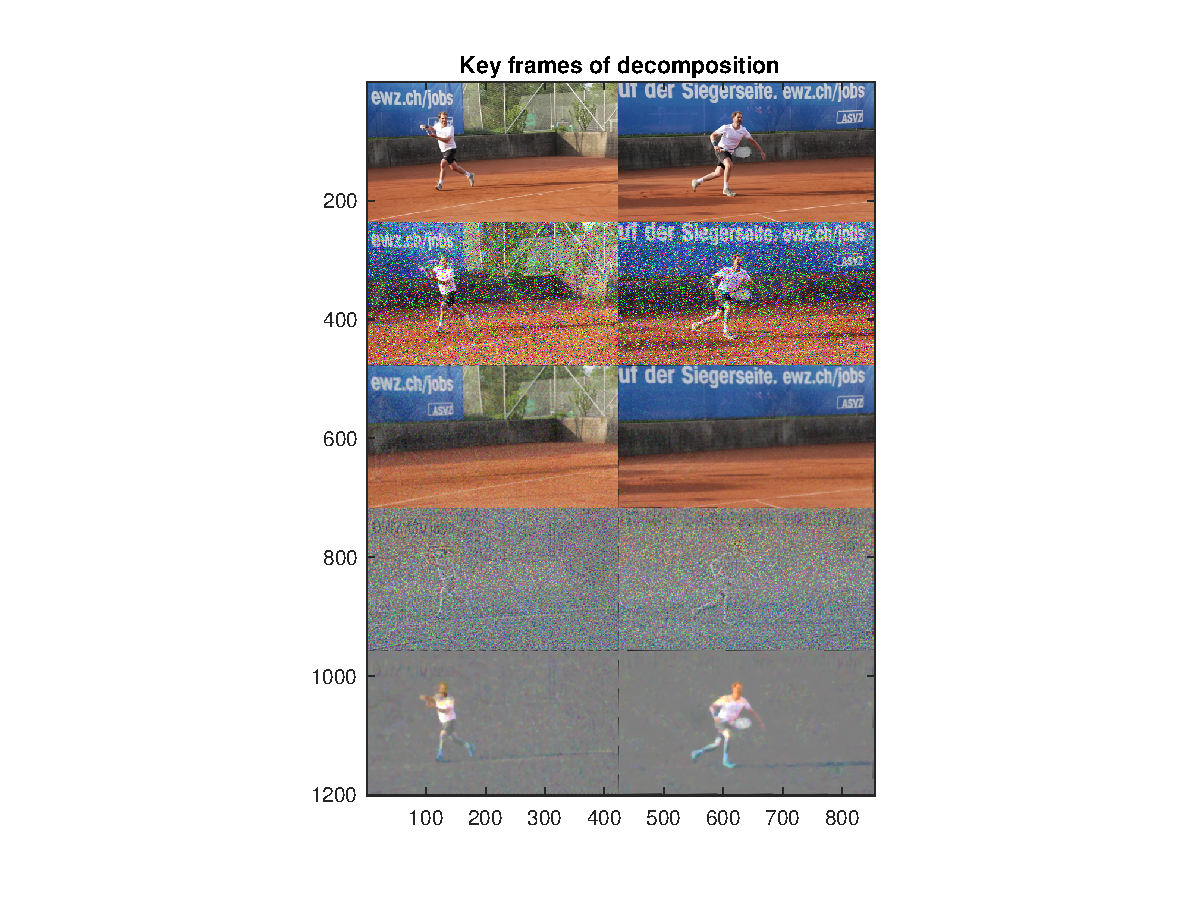
\includegraphics[trim=5.8cm 1.5cm 5cm 1.1cm,clip=true, width=0.33\textwidth]{tennis.eps}}
\subfigure{\includegraphics[trim=5.8cm 1.5cm 5cm 1.1cm,clip=true,width=0.33\textwidth]{paragliding.eps}}
\subfigure{\includegraphics[trim=5.8cm 1.5cm 5cm  1.1cm,clip=true,width=0.33\textwidth]{horsejump-high.eps}}
\caption{PanGAEA separation results on DAVIS Challenge 2017 videos \cite{DAVIS}. From top to bottom: Original frames, Corrupted frames with 20\% shotgun noise (Observed), Recovered Background, Recovered Sparse Corruptions, Recovered Foreground. Left to right: ``Tennis",``Paragliding", ``Horsejump-High".}
    \label{fig:decomp-frames}
    \end{center}
\end{figure*}

\begin{figure*}
\centering
    \subfigure[``Tennis" Clean]{\includegraphics[trim=0cm 0cm 0cm 1cm,clip=true,width=0.3\textwidth]{tennis_roc_clean.eps}}
    \subfigure[``Paragliding" Clean]{\includegraphics[trim=0cm 0cm 0cm 1cm,clip=true,width=0.3\textwidth]{paragliding_roc_clean.eps}}
    \subfigure[``Horsejump-High" Clean]{\includegraphics[trim=0cm 0cm 0cm 1cm,clip=true,width=0.3\textwidth]{horsejump-high_roc_clean.eps}}
    \vfill
    \subfigure[``Tennis" Corrupted]{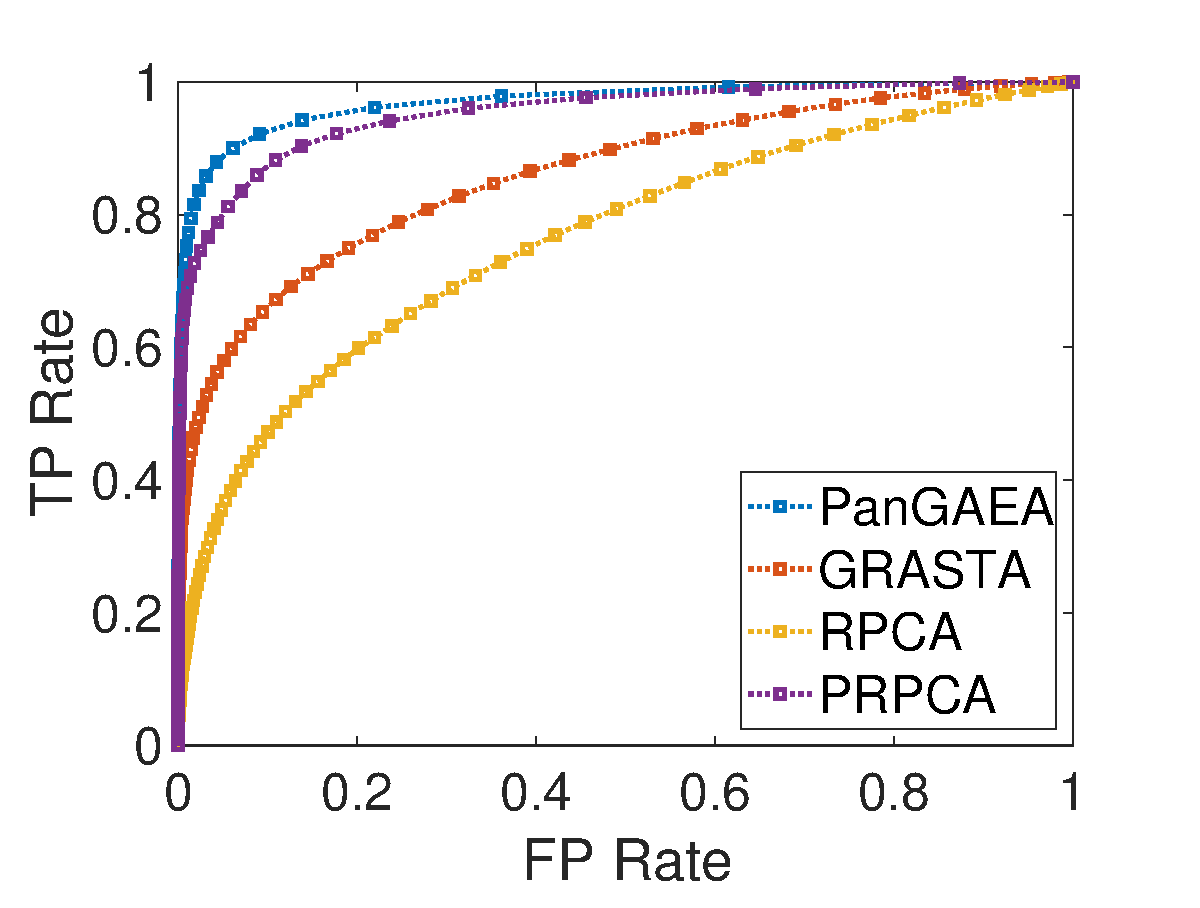
\includegraphics[trim=0cm 0cm 0cm 1cm,clip=true,width=0.3\textwidth]{tennis_roc_corrupted.eps}}
    \subfigure[``Paragliding" Corrupted]{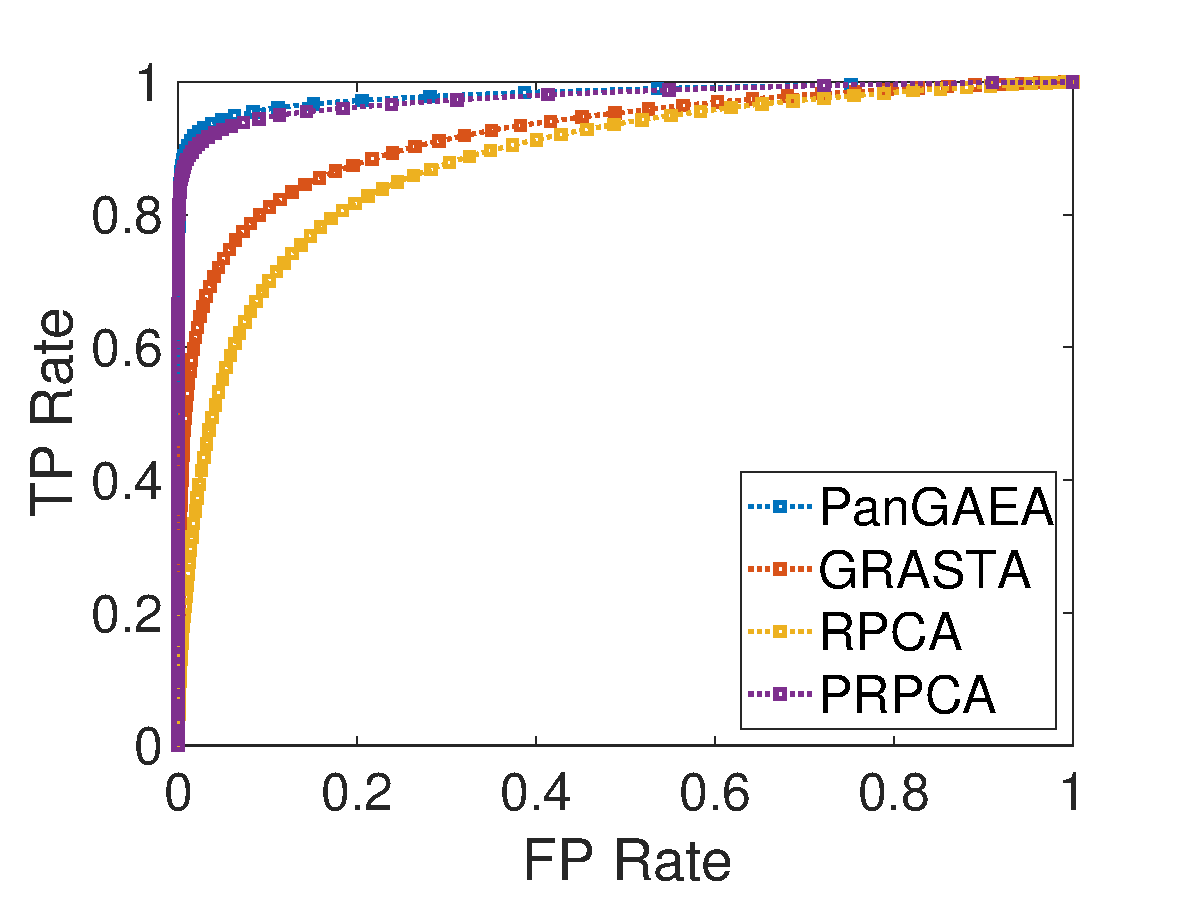
\includegraphics[trim=0cm 0cm 0cm 1cm,clip=true,width=0.3\textwidth]{paragliding_roc_corrupted.eps}}
    \subfigure[``Horsejump-High" Corrupted]{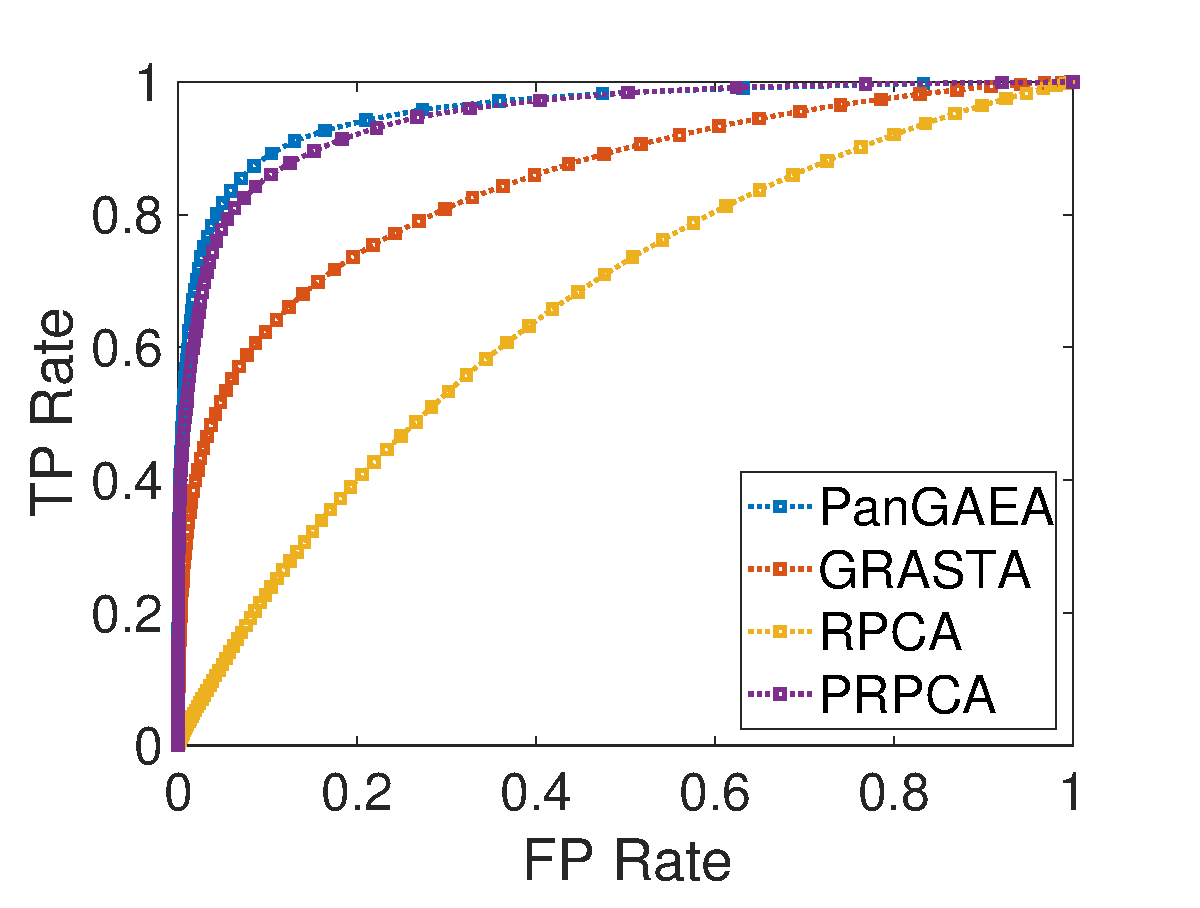
\includegraphics[trim=0cm 0cm 0cm 1cm,clip=true,width=0.3\textwidth]{horsejump-high_roc_corrupted.eps}}
    \caption{ROC curves for ``Tennis". PanGAEA achieves the largest area under its curve in both clean and noisy video and outperforms its competitors. }
    \label{fig:tennis_roc}
\end{figure*}



% \begin{figure*}
%     \centering
    
%     \subfloat[``Tennis": Clean]{\includegraphics[trim=0cm 0cm 0cm 1cm,clip=true,width=0.3\textwidth]{tennis_roc_clean.eps}} \quad
%     \subfloat[``Paragliding": Clean]{\includegraphics[trim=0cm 0cm 0cm 1cm,clip=true,width=0.3\textwidth]{paragliding_roc_clean.eps}} 
%     \subfloat[``Horsejump-High":Clean]{\includegraphics[trim=0cm 0cm 0cm 1cm,clip=true, width=0.3\textwidth]{horsejump-high_roc_clean.eps}} \quad
%     \subfloat[``Tennis": Corrupted]{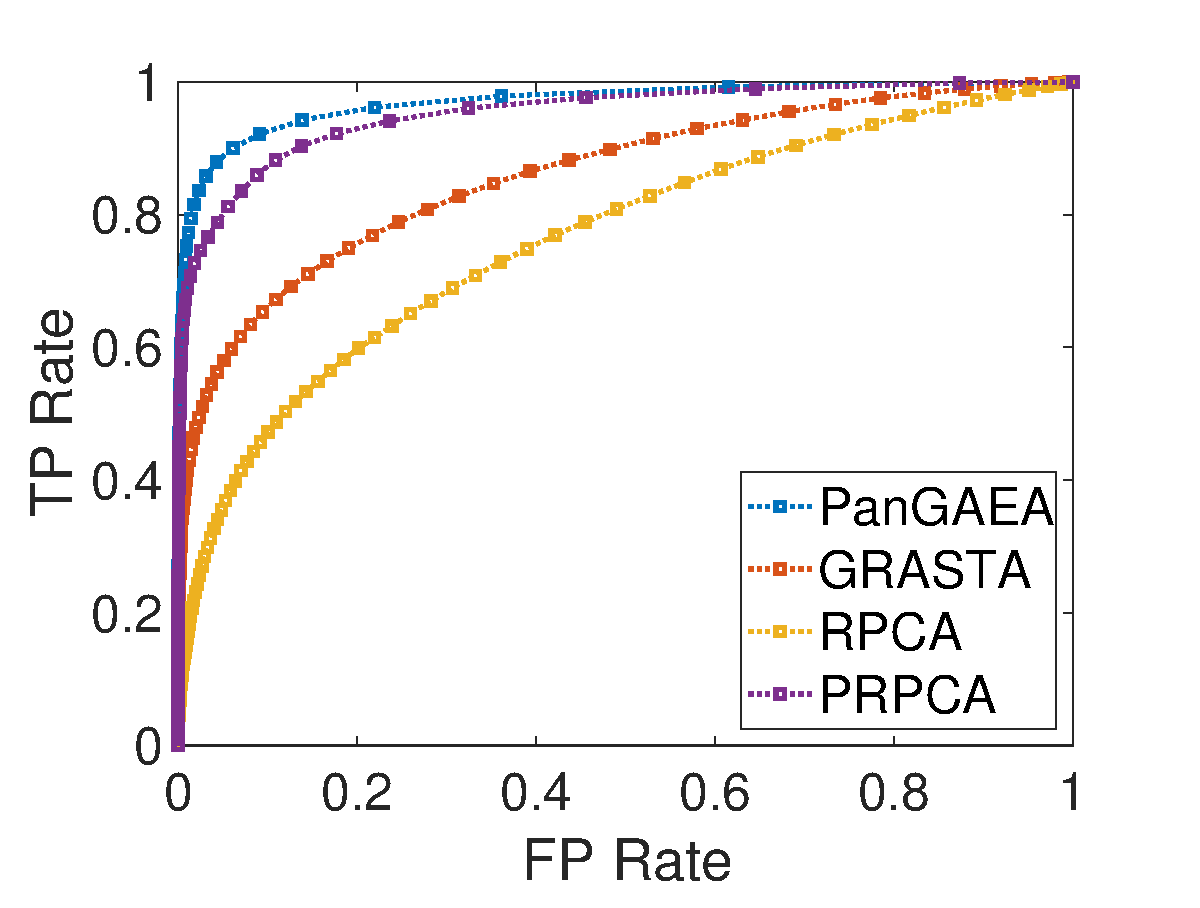
\includegraphics[trim=0cm 0cm 0cm 1cm,clip=true,width=0.3\textwidth]{tennis_roc_corrupted.eps}} 
%     \subfloat[``Paragliding": Corrupted]{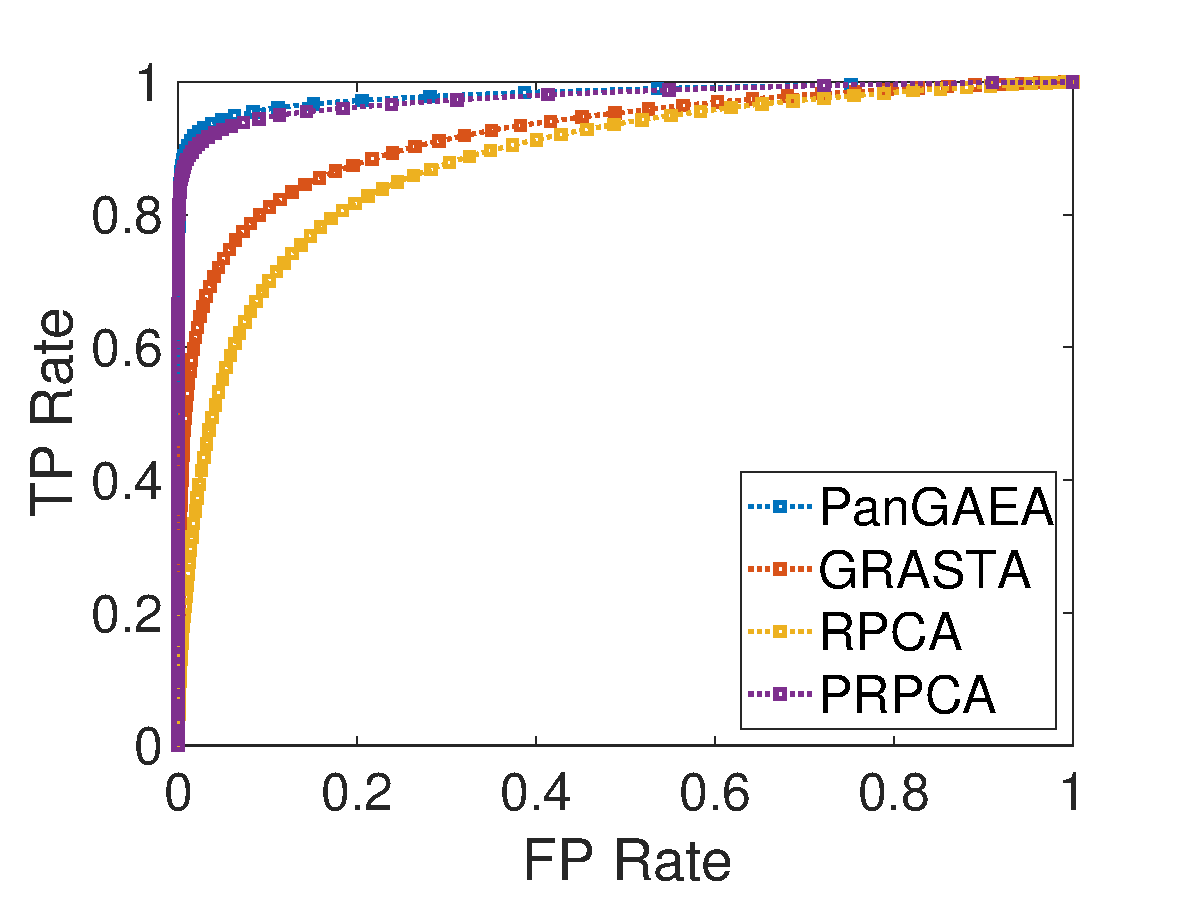
\includegraphics[trim=0cm 0cm 0cm 1cm,clip=true,width=0.3\textwidth]{paragliding_roc_corrupted.eps}}
%     \subfloat[``Horsejump-High": Corrupted]{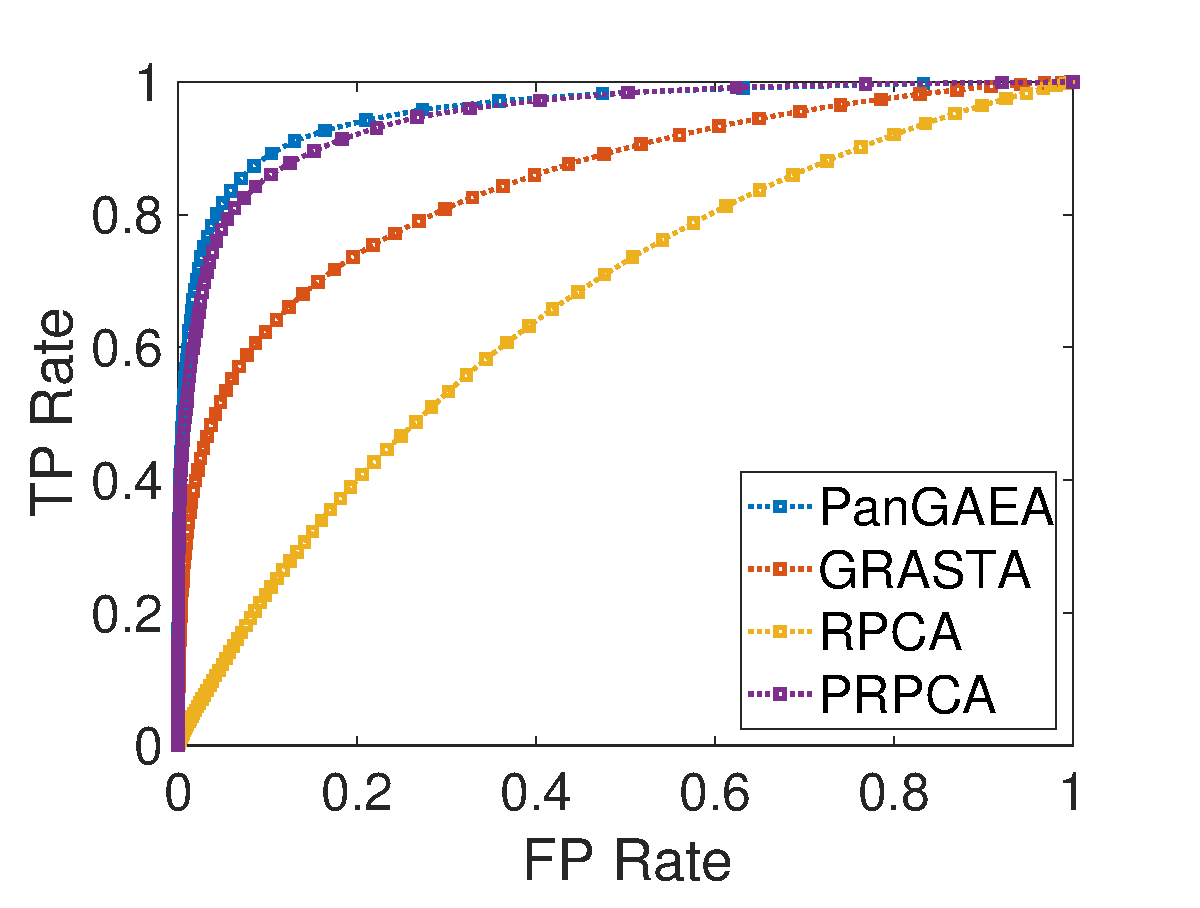
\includegraphics[trim=0cm 0cm 0cm 1cm,clip=true,width=0.3\textwidth]{horsejump-high_roc_corrupted.eps}}
%     \caption{ROC curves for ``Tennis". PanGAEA achieves the largest area under its curve in both clean and noisy video and outperforms its competitors. }
%     \label{fig:tennis_roc}
% \end{figure*}


\section{Conclusions and Future Work} \label{section:conclusions}

In this paper we have presented a novel TV-regularized RPCA algorithm that can estimate subspaces on the Grassmann manifold and perform foreground-background separation in panoramic video. Our algorithm achieves competitive performance with PRPCA in far less computational time by performing first-order gradient descent on the Grassmann manifold. PanGAEA is an online method by nature and can be applied to problems with streaming vector data. 

Our future work aims to make the panoramic RPCA problem truly online where the geometric transformation between frames is estimated in the objective function on the fly as the frames are captured by the camera. We also seek an adaptive step size like the one proposed for GRASTA in \cite{grasta} so that PanGAEA may track time-dynamical subspaces in an online setting. Also of key interest to us is making our algorithm robust to dense Gaussian or Poisson noise and imputing missing values of the sparse components, since our method can only complete the low-rank background from partial information.

\newpage
{\small
\bibliographystyle{ieee}
\bibliography{references.bib}
}

\end{document}
